% Digital Logic Report Template
% Created: 2020-04-01, Ashlie Lackey

%==========================================================
%=========== Document Setup  ==============================

% Formatting defined by class file
\documentclass[11pt]{article}

% ---- Document formatting ----
\usepackage[margin=1in]{geometry}	% Narrower margins
\usepackage{booktabs}				% Nice formatting of tables
\usepackage{graphicx}				% Ability to include graphics

%\setlength\parindent{0pt}	% Do not indent first line of paragraphs 
\usepackage[parfill]{parskip}		% Line space b/w paragraphs
%	parfill option prevents last line of pgrph from being fully justified

% Parskip package adds too much space around titles, fix with this
\RequirePackage{titlesec}
\titlespacing\section{0pt}{8pt plus 4pt minus 2pt}{3pt plus 2pt minus 2pt}
\titlespacing\subsection{0pt}{4pt plus 4pt minus 2pt}{-2pt plus 2pt minus 2pt}
\titlespacing\subsubsection{0pt}{2pt plus 4pt minus 2pt}{-6pt plus 2pt minus 2pt}

% ---- Hyperlinks ----
\usepackage[colorlinks=true,urlcolor=blue]{hyperref}	% For URL's. Automatically links internal references.

% ---- Code listings ----
\usepackage{listings} 					% Nice code layout and inclusion
\usepackage[usenames,dvipsnames]{xcolor}	% Colors (needs to be defined before using colors)

% Define custom colors for listings
\definecolor{listinggray}{gray}{0.98}		% Listings background color
\definecolor{rulegray}{gray}{0.7}			% Listings rule/frame color

% Style for Verilog
\lstdefinestyle{Verilog}{
	language=Verilog,					% Verilog
	backgroundcolor=\color{listinggray},	% light gray background
	rulecolor=\color{blue}, 			% blue frame lines
	frame=tb,							% lines above & below
	linewidth=\columnwidth, 			% set line width
	basicstyle=\small\ttfamily,	% basic font style that is used for the code	
	breaklines=true, 					% allow breaking across columns/pages
	tabsize=3,							% set tab size
	commentstyle=\color{gray},	% comments in italic 
	stringstyle=\upshape,				% strings are printed in normal font
	showspaces=false,					% don't underscore spaces
}

% How to use: \Verilog[listing_options]{file}
\newcommand{\Verilog}[2][]{%
	\lstinputlisting[style=Verilog,#1]{#2}
}




%======================================================
%=========== Body  ====================================
\begin{document}

\title{ELC 2137 Lab 9: ALU with Input Register}
\author{Ashlie Lackey}

\maketitle


\section*{Summary}

The goal of this lab was to start on building a small calculator by creating an ALU and using two registers to do some mathematical operations including: addition, subtraction, AND, OR, and XOR, along with a default that returns in0. The registers are used to store the numbers when inputting, as one input comes from the switches and the other comes from the register in which it is stored. Additionally, the switches are also used to specify which operation is to be performed. During this lab skills were gained to learn the differences between combinational and sequential logic and how to implement in Verilog, understanding and some implementation of SR latches, D latches, D flip flops, and D registers, and reuse of modules from previous labs. 

\section*{Results}

Simulation waveforms, expected results tables, and pictures of the operations testing on the Basys3 board are included below to demonstrate that the ALU built during this lab works correctly.

\subsection*{Expected results tables}
\begin{table*}[ht]\centering
	\caption{\textit{register} expected results table}
	\label{ALU:tbl:register_ERT}\medskip
	\begin{tabular}{l|rrrrrrrrrrr}
		Time (ns): & 0-5 & 5-10 & 10-15 & 15-20 & 20-25 & 25-30 & 30-35 & 35-40& 40-45 & 45-50 & 50-55 \\
		\midrule
		D (hex) & 0 & 0     & A & A & 3         & 3       & 0           & 0 & 0$\to$6 & 6 & 6 \\
		clk     & 0 & 1     & 0 & 1 & 0         & 1       & 0           & 1 & 0   & 1 & 0 \\
		en    & 0 & 0       & 1 & 1 & 1$\to$0 & 0$\to$1 & 1$\to$0 & 0 & 0$\to$1& 1 & 1 \\
		rst   & 0 & 0$\to$1 & 0 & 0 & 0          & 0     & 0       & 0 & 0  & 0 & 0 \\
		\midrule
		Q (hex) & X & X$\to$0 & 0 & A & A & A & A & A & A & 6 & 6 \\
		\bottomrule
	\end{tabular}
\end{table*}

\begin{table*}[ht]\centering
	\caption{\textit{alu} expected results table skeleton}
	\label{ALU:tbl:alu_ERT}\medskip
	\begin{tabular}{l|rrrrrr}
		Time (ns): & 0-10 & 10-20 & 20-30 & 30-40 & 40-50 & 50-60 \\
		\midrule
		in0 & 14  & 14 & 14 & 14 & 14 & 14 \\
		in1 & 7A & 7A & 7A & 7A & 7A & 7A \\
		op    & default & ADD(0) & SUB(1) & AND(2) & OR(3) & XOR(4) \\
		\midrule
		out & 14 & 8E & 9A & 10 & 7E & 6E \\
		\bottomrule
	\end{tabular}
\end{table*}
\clearpage

\subsection*{Simulation Waveforms}
\begin{figure}[ht]\centering
	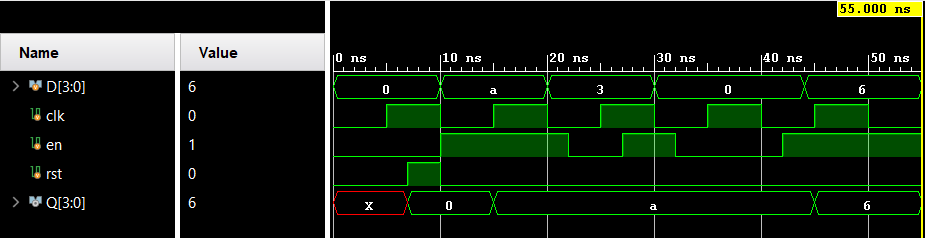
\includegraphics[width=1\textwidth]{register_test}
	\caption{\textit{register testbench} Simulation Waveform}
	\label{fig:sim_with_table}
\end{figure}

\begin{figure}[ht]\centering
	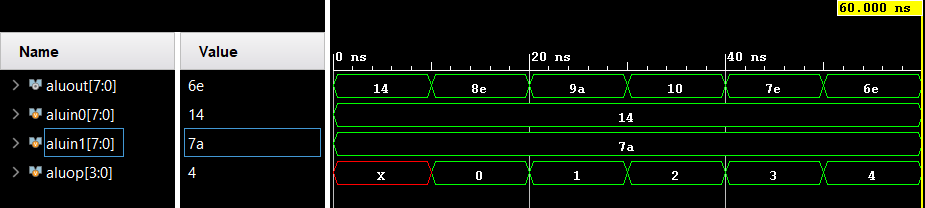
\includegraphics[width=1\textwidth]{alu_test}
	\caption{\textit{ALU testbench} Simulation Waveform}
	\label{fig:sim_with_table}
\end{figure}
\clearpage

\subsection*{Operation On-board Testing}

NOTE: 7A was the initial input for the subtraction test to keep the outputs consistent with the ALU testbench simulation outputs.

\begin{figure}[ht]\centering
	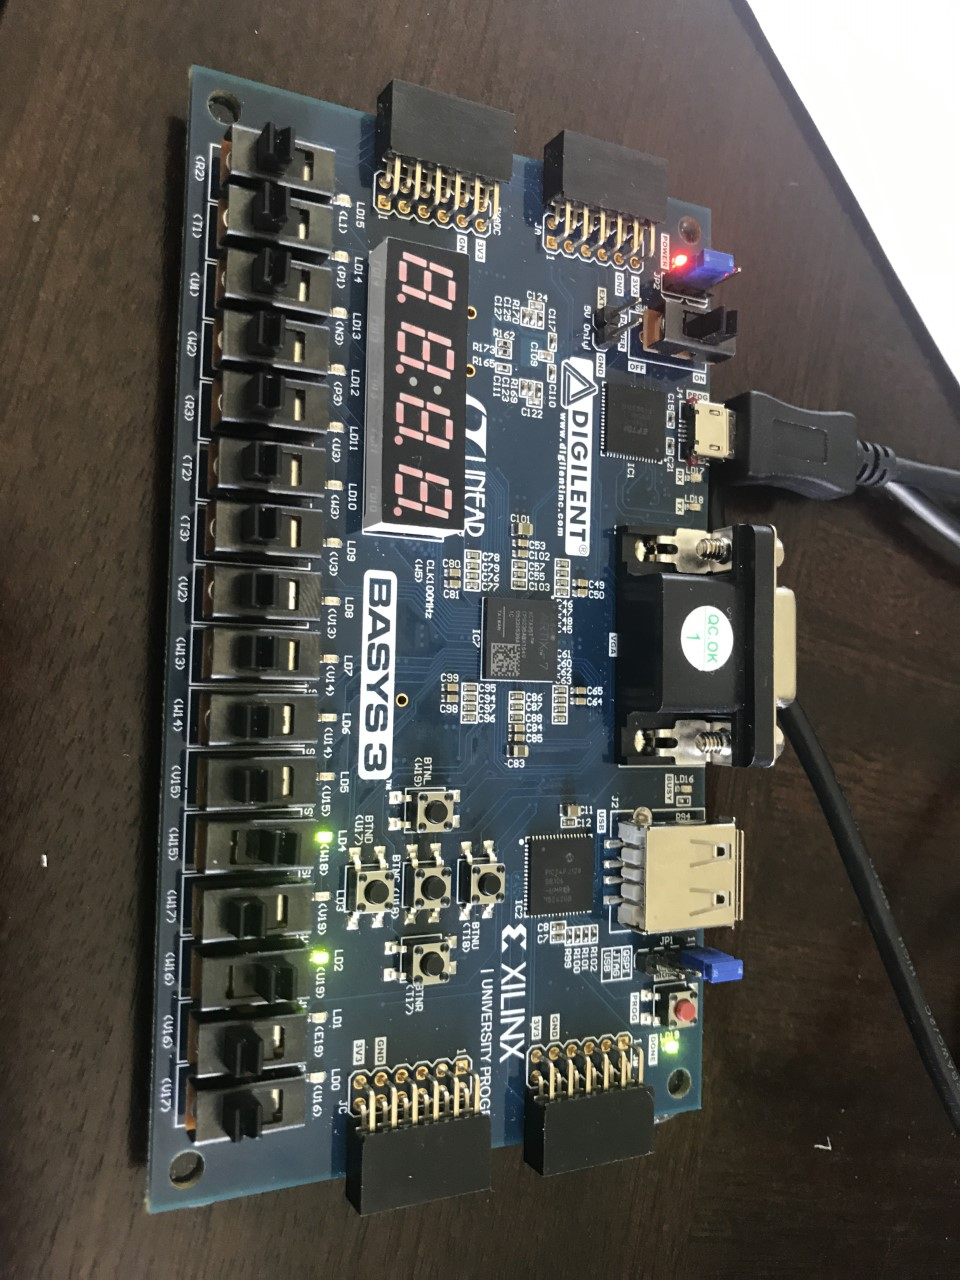
\includegraphics[angle=90, width=.8\textwidth]{default1}
	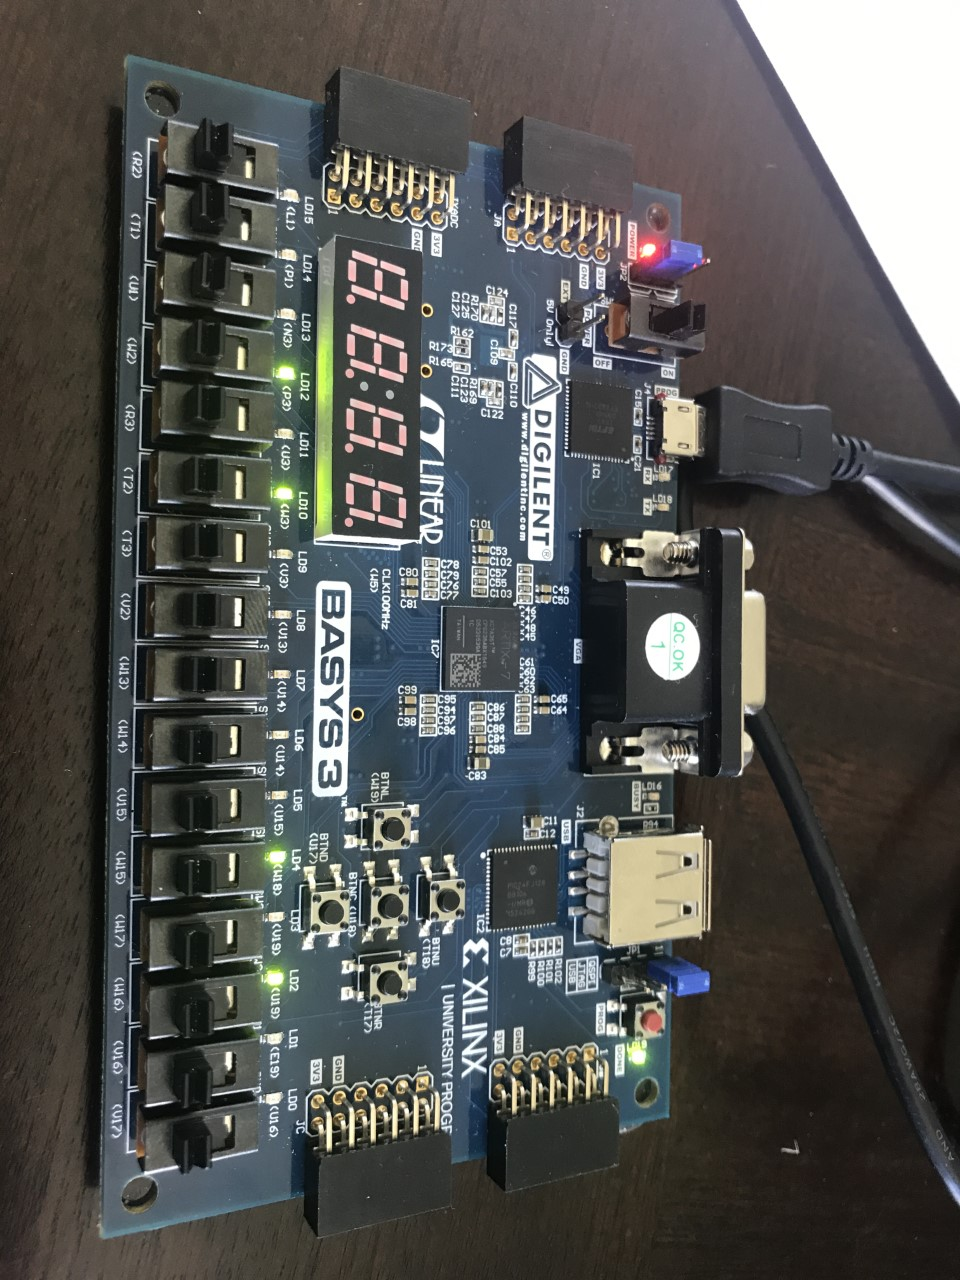
\includegraphics[angle=90, width=.8\textwidth]{default2}
	\caption{\textit{default} Board Test}
	\label{fig:sim_with_table}
\end{figure}

\begin{figure}[ht]\centering
	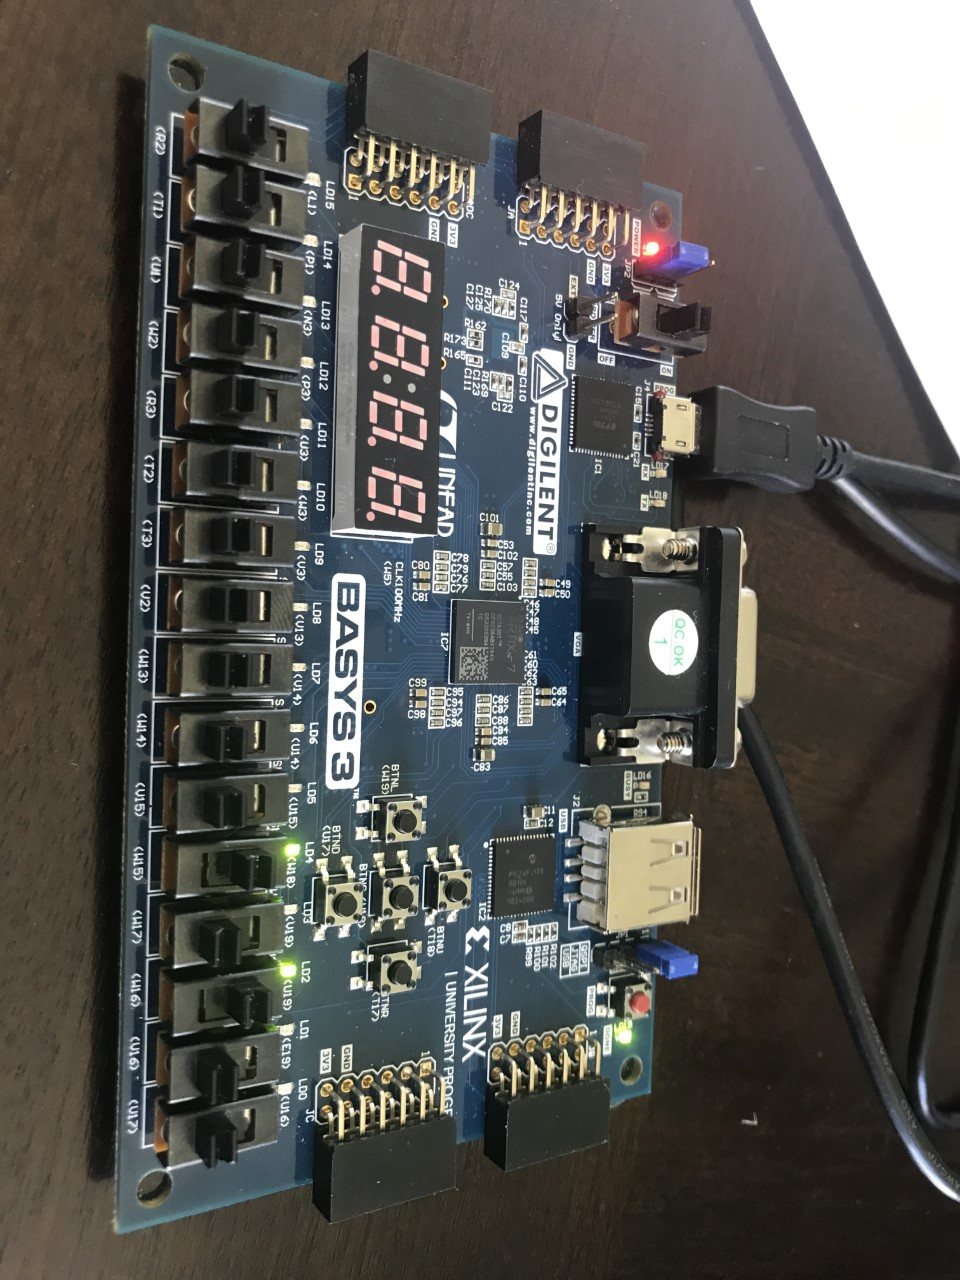
\includegraphics[angle=90, width=.8\textwidth]{add1}
	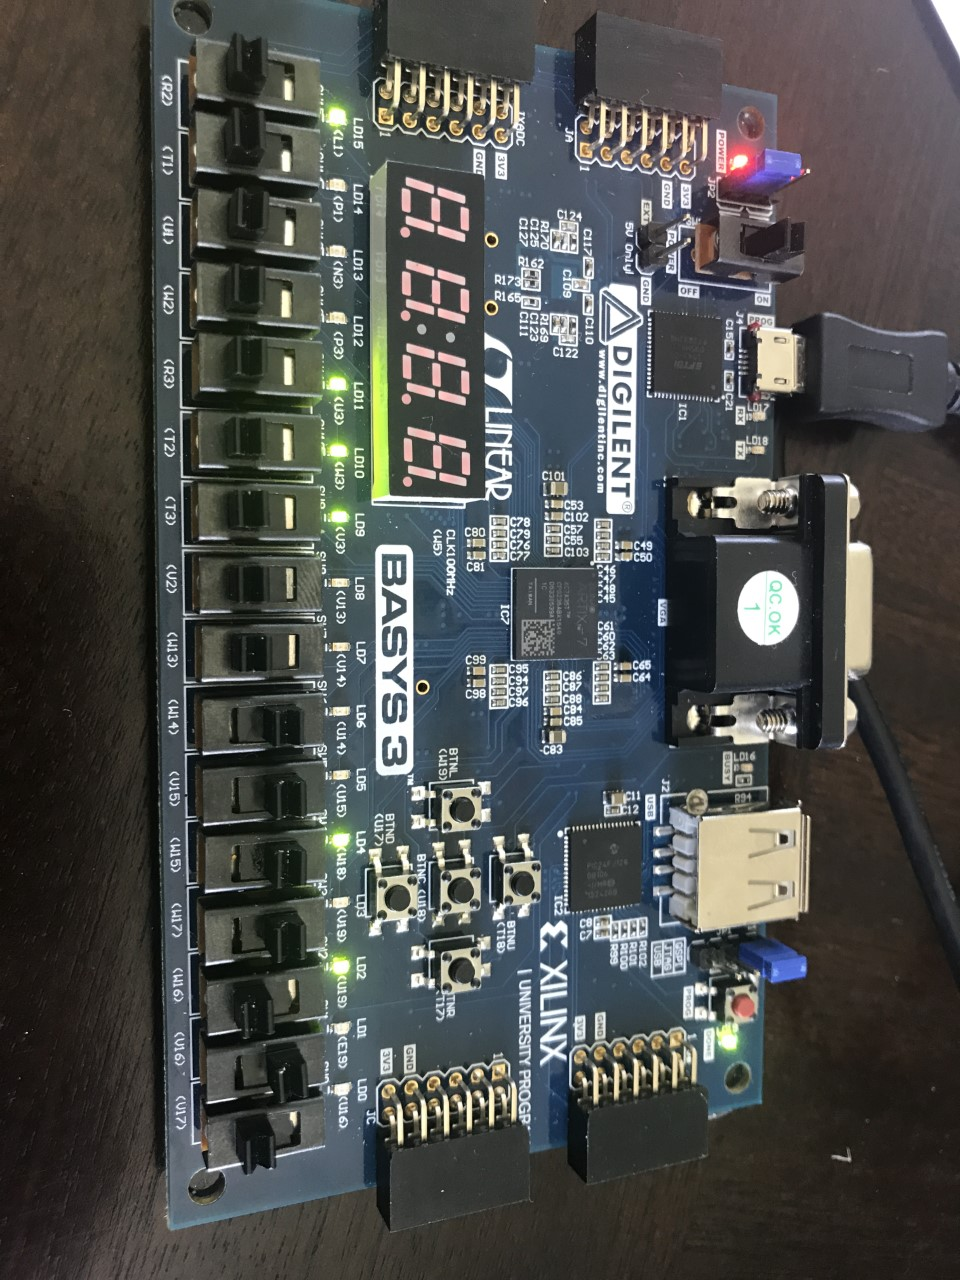
\includegraphics[angle=90, width=.8\textwidth]{add2}
	\caption{\textit{add} Board Test}
	\label{fig:sim_with_table}
\end{figure}

\begin{figure}[ht]\centering
	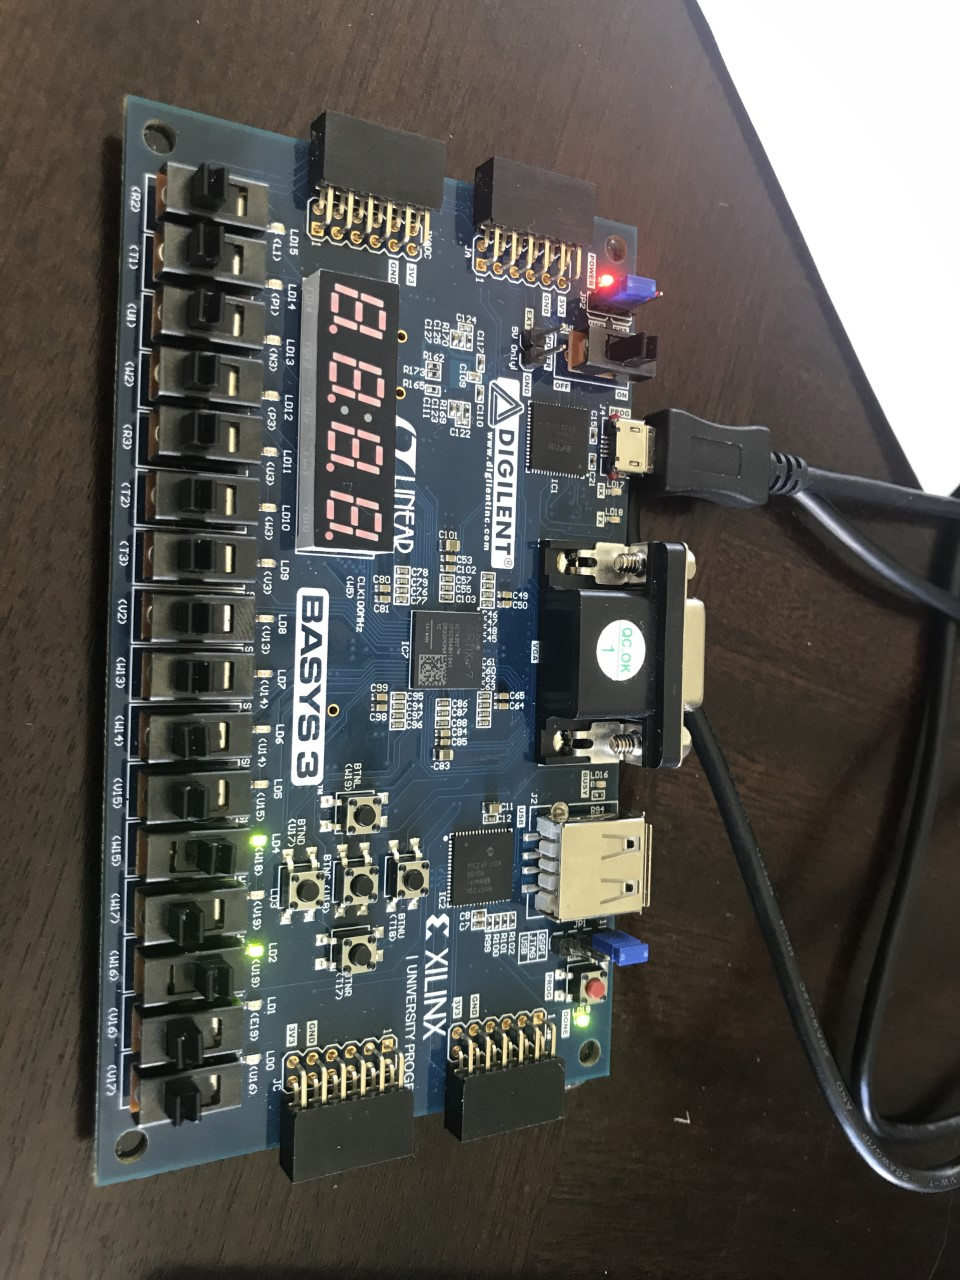
\includegraphics[angle=90, width=.8\textwidth]{sub1}
	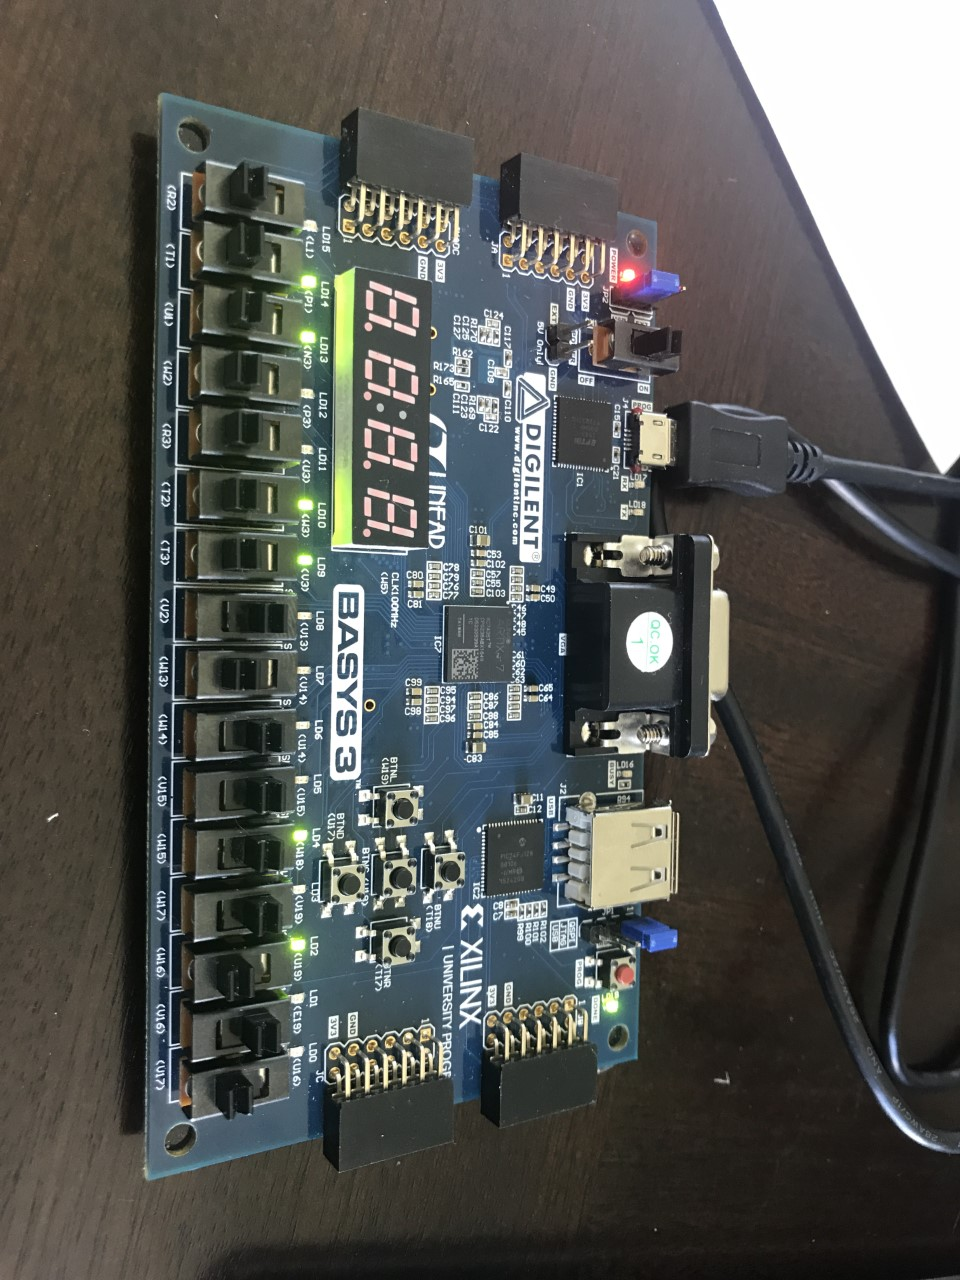
\includegraphics[angle=90, width=.8\textwidth]{sub2}
	\caption{\textit{subtract} Board Test}
	\label{fig:sim_with_table}
\end{figure}

\begin{figure}[ht]\centering
	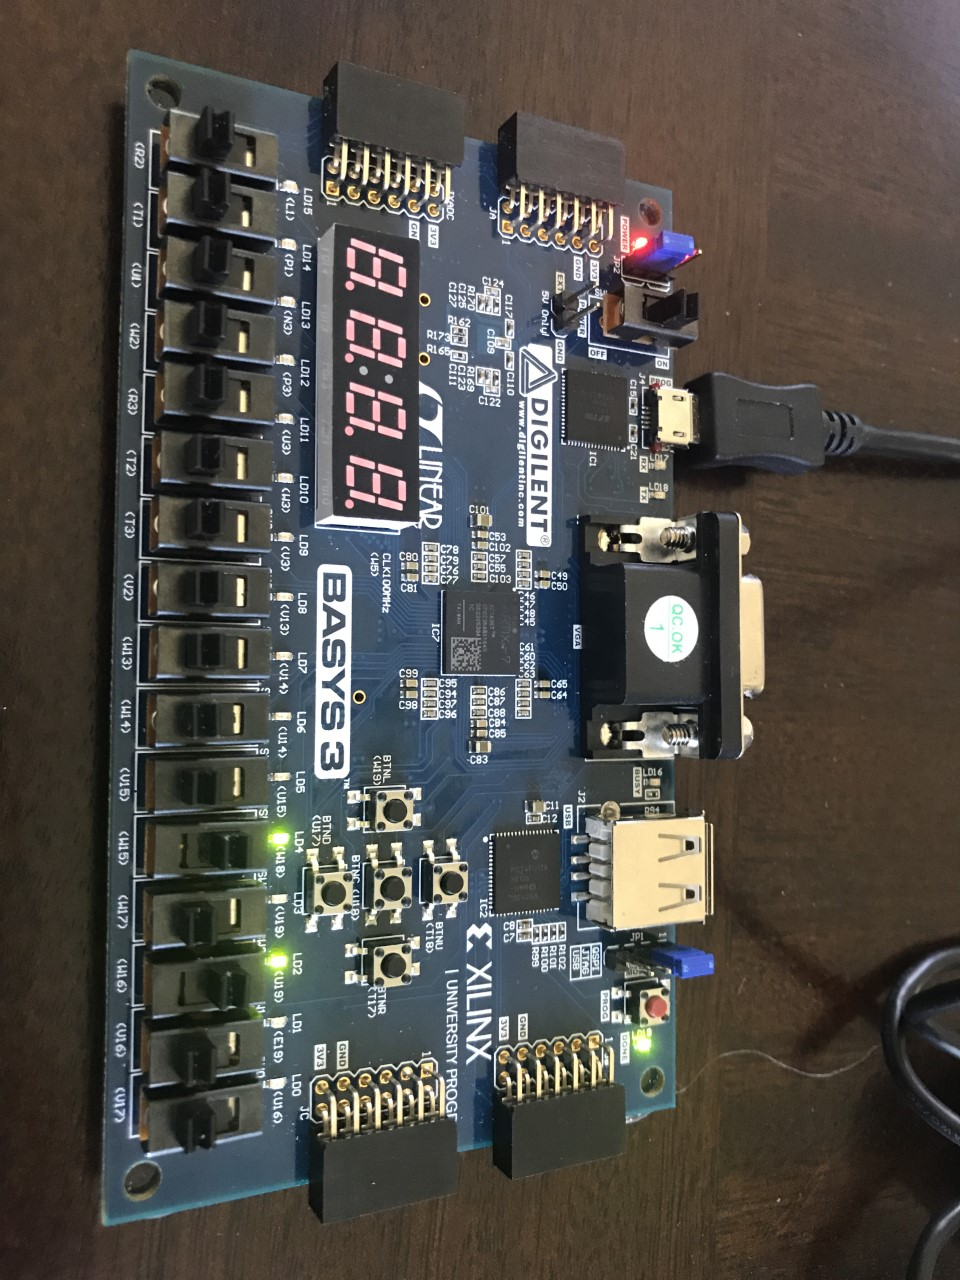
\includegraphics[angle=90, width=.8\textwidth]{and1}
	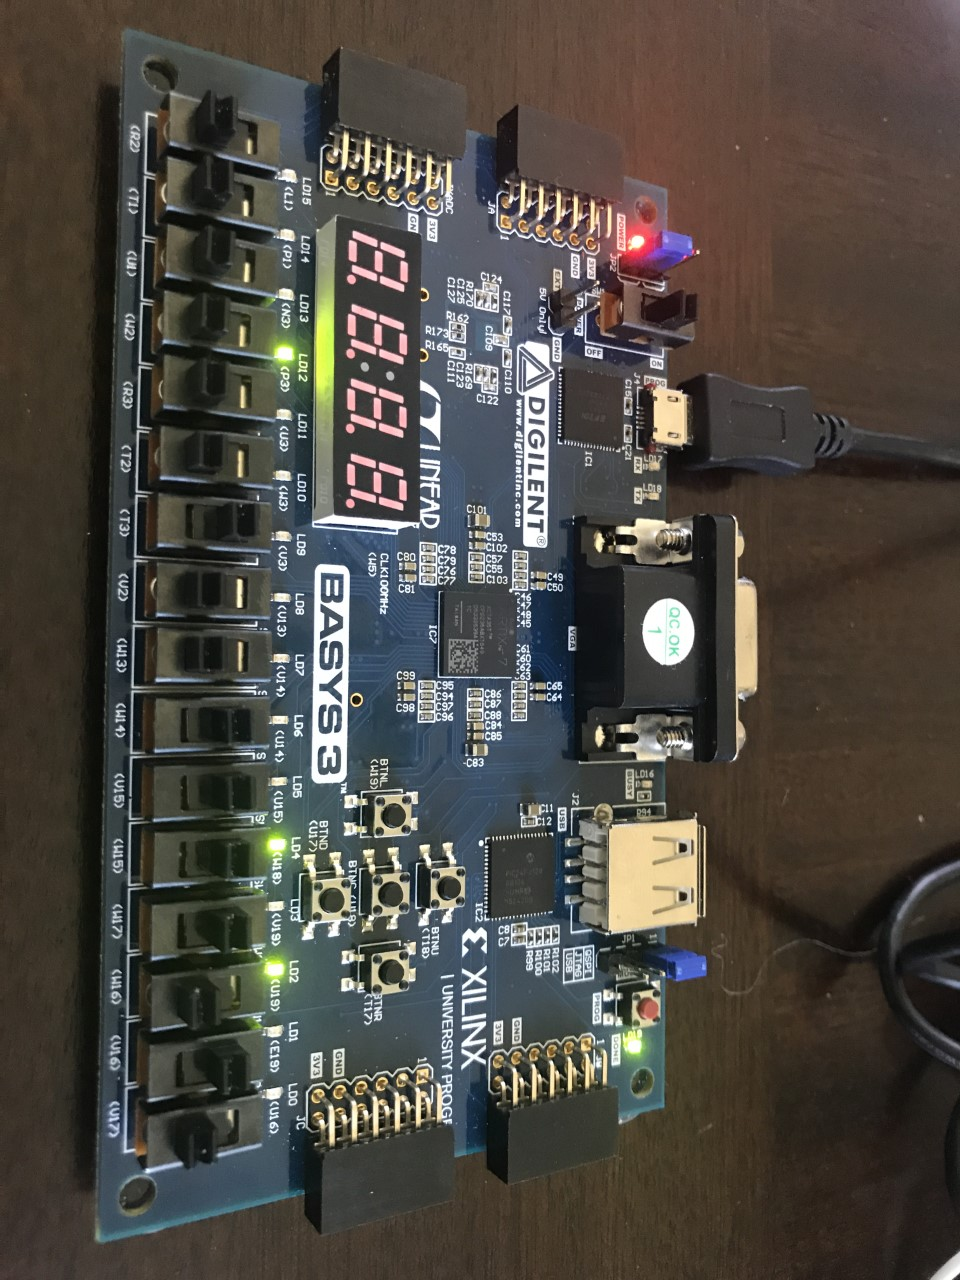
\includegraphics[angle=90, width=.8\textwidth]{and2}
	\caption{\textit{AND} Board Test}
	\label{fig:sim_with_table}
\end{figure}

\begin{figure}[ht]\centering
	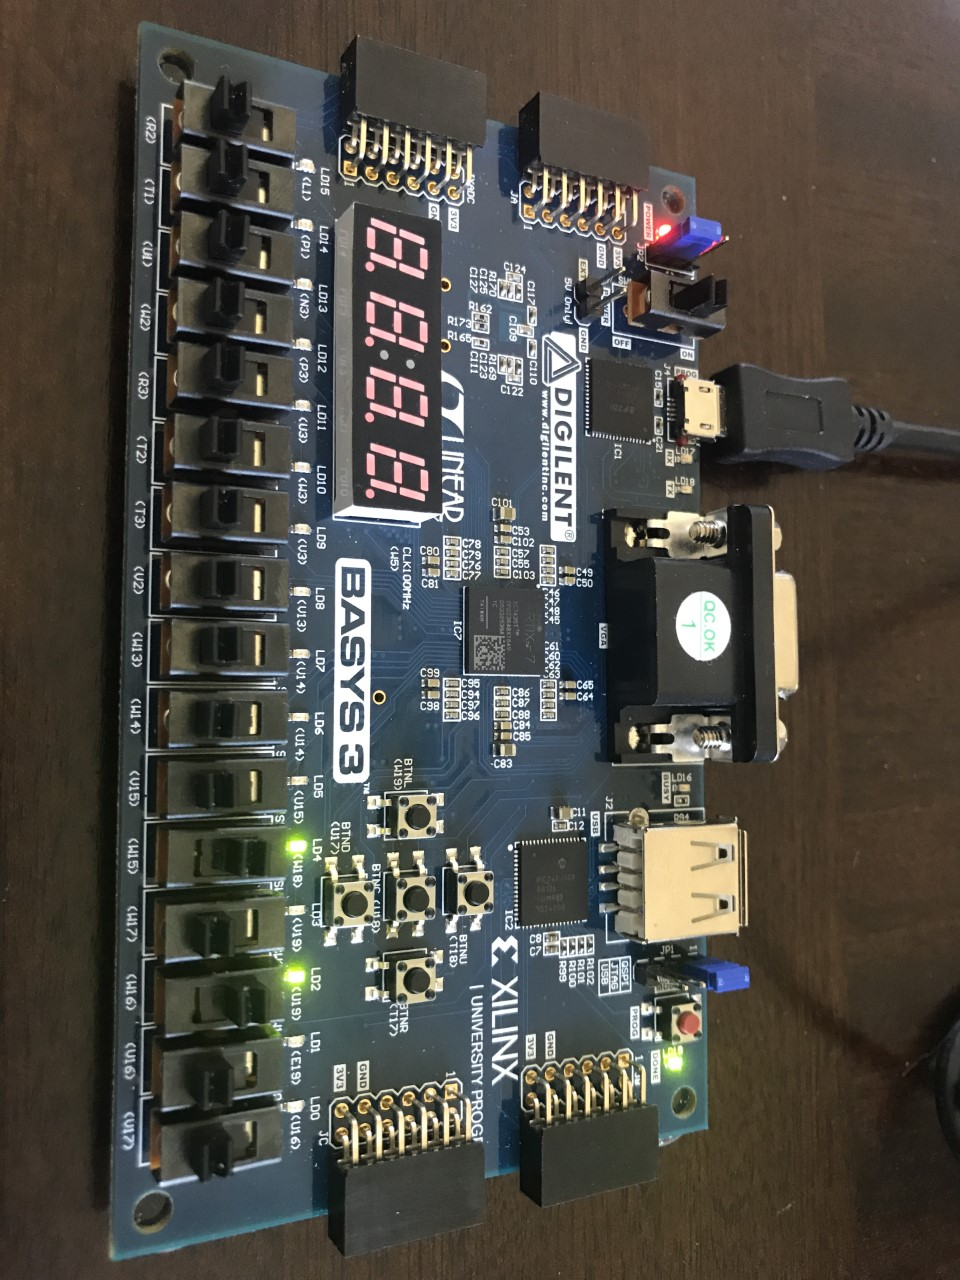
\includegraphics[angle=90, width=.8\textwidth]{or1}
	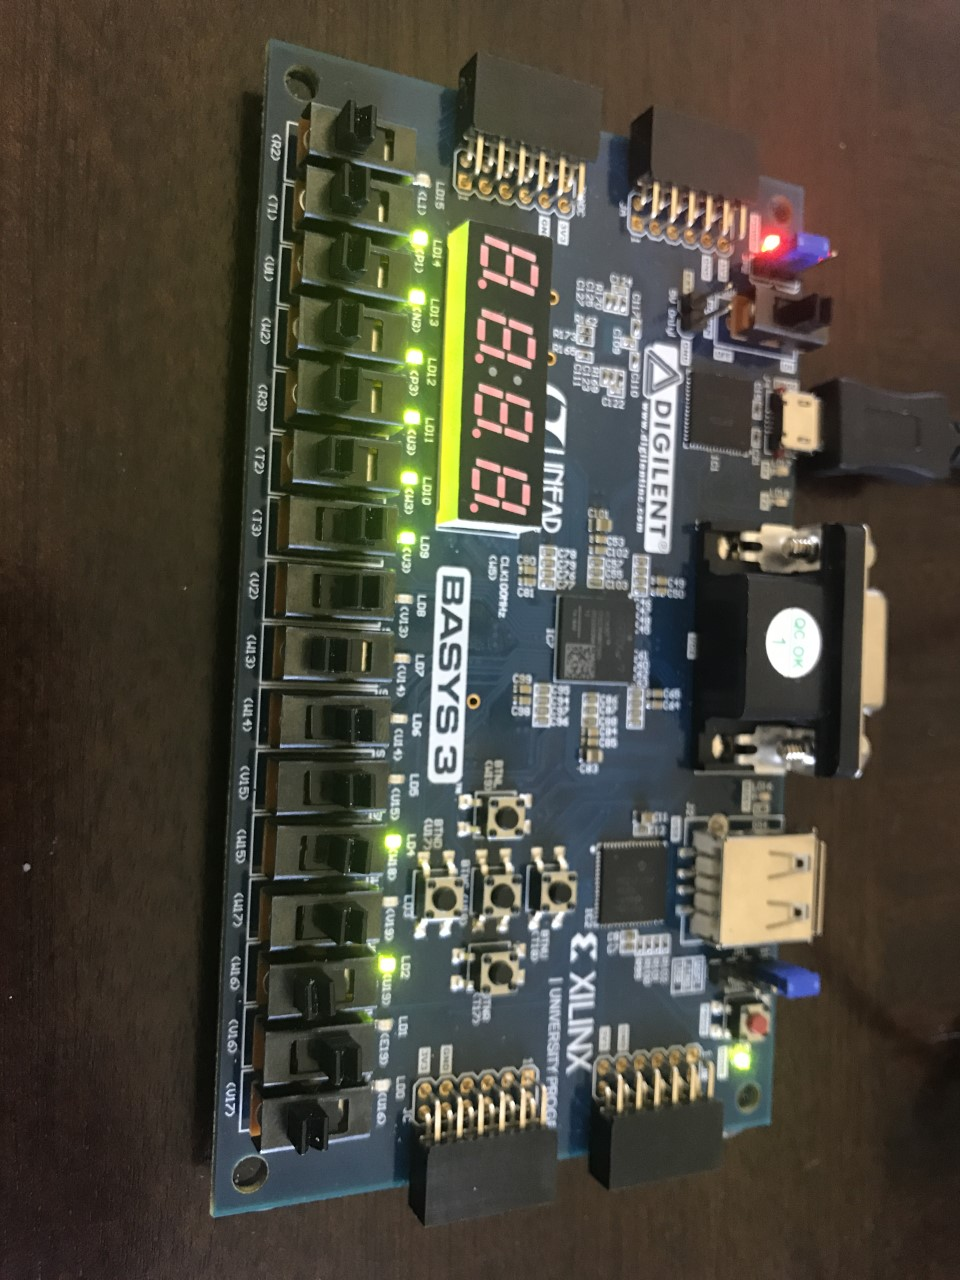
\includegraphics[angle=90, width=.8\textwidth]{or2}
	\caption{\textit{OR} Board Test}
	\label{fig:sim_with_table}
\end{figure}

\begin{figure}[ht]\centering
	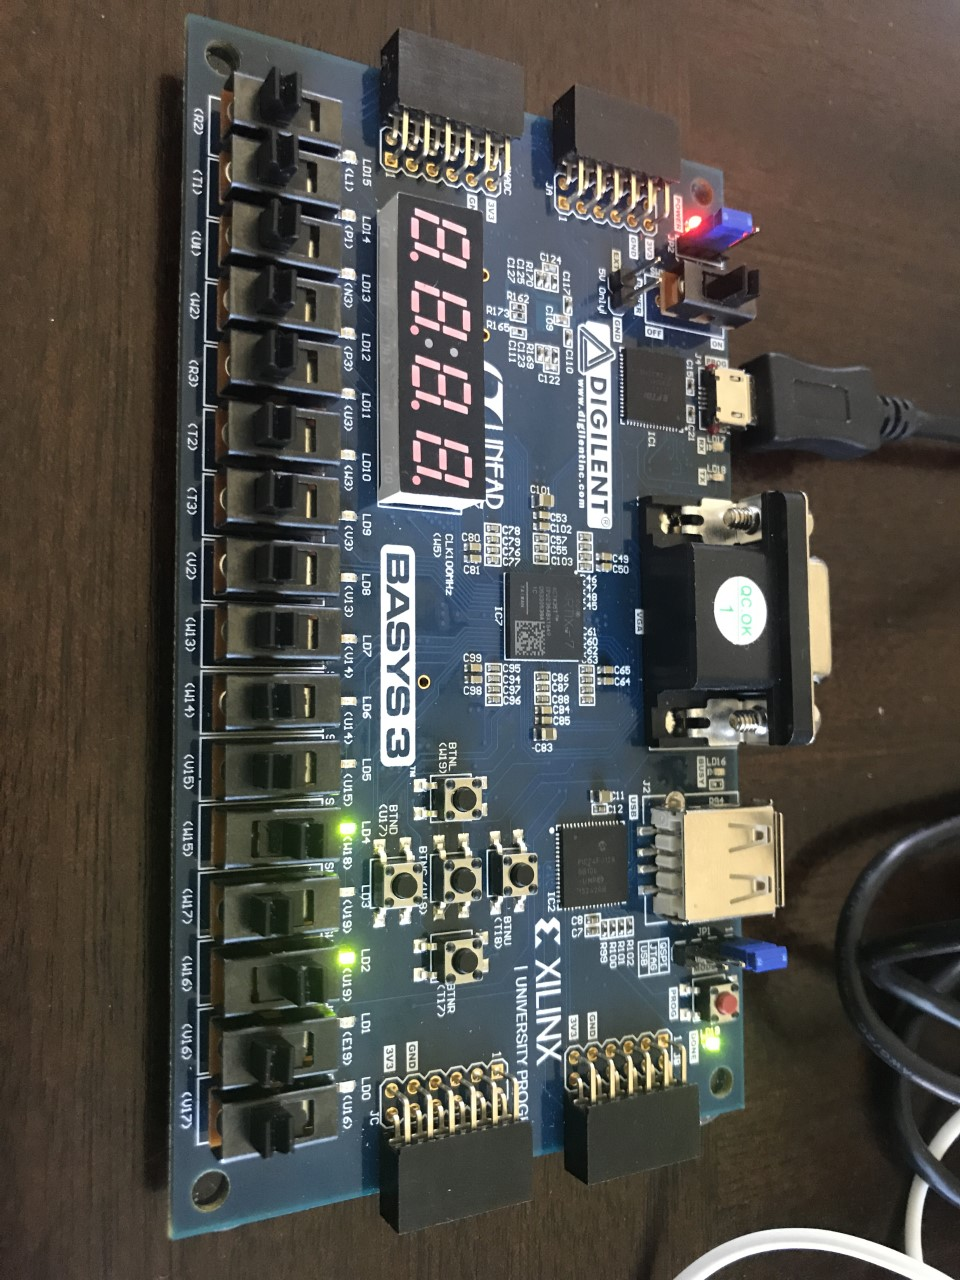
\includegraphics[angle=90, width=.8\textwidth]{xor1}
	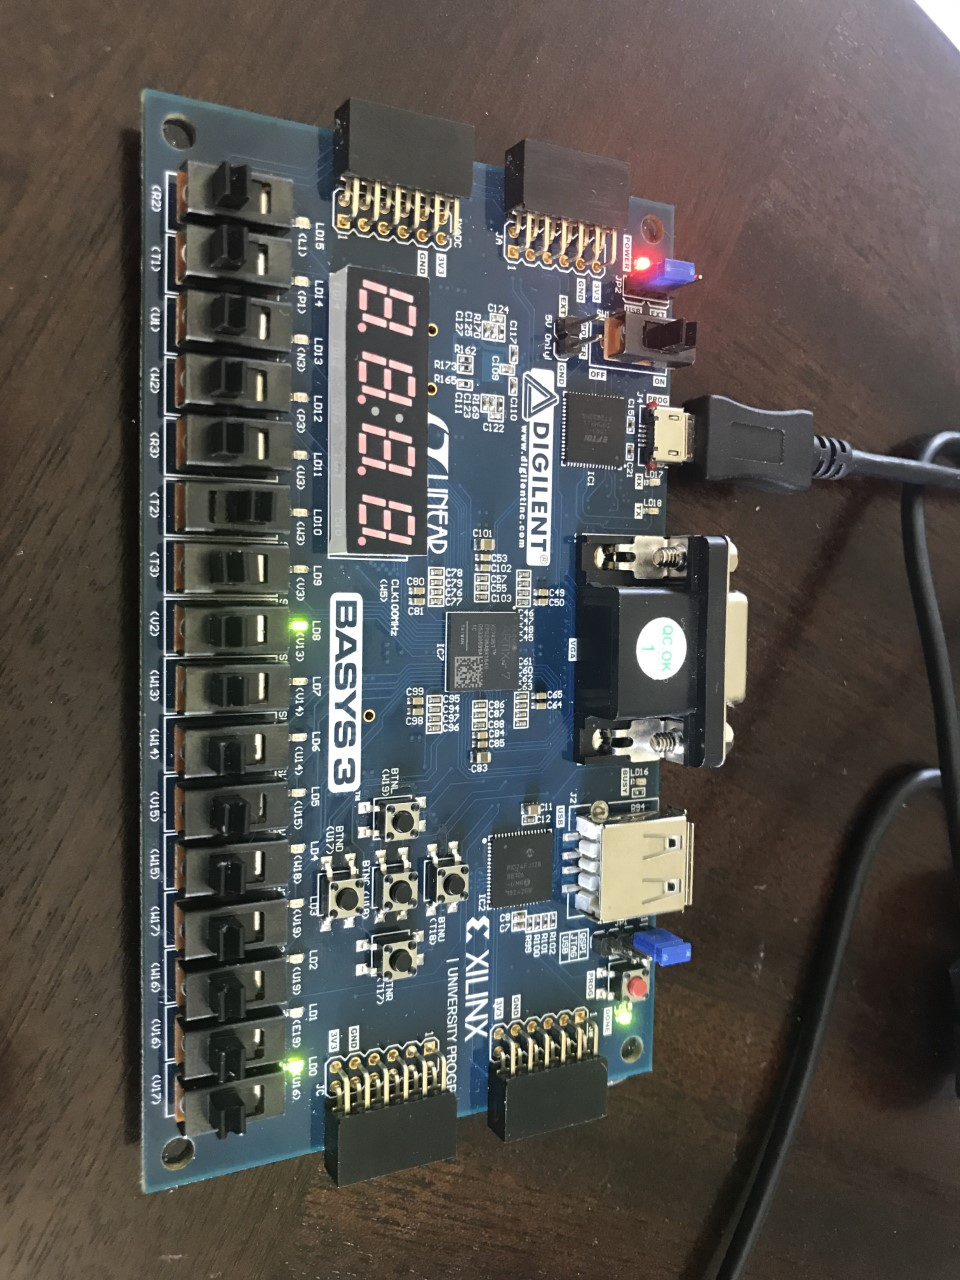
\includegraphics[angle=90, width=.8\textwidth]{xor2}
	\caption{\textit{XOR} Board Test}
	\label{fig:sim_with_table}
\end{figure}
\clearpage

\section*{Code}

\begin{lstlisting}[style=Verilog,caption= register Verilog Code,label=code:ex ]
`timescale 1ns / 1ps
// Ashlie Lackey, ELC 2137, 2020 -03 -26
module  register  #( parameter N=1)
	(input clk , rst , en ,
	input [N -1:0] D,
	output  reg [N -1:0] Q);
	
	always @(posedge clk , posedge  rst)
	begin
	if (rst ==1)
		Q <= 0;
	else if (en==1)
		Q <= D;
	end
	
	// Notes:
	// - Reset  is  asynchronous , so this
	//    block  needs  to  execute  when  rst
	//    goes  high.
	// - We want  enable  to be  synchronous
	//    (i.e. only  happens  on  rising
	//    edge of clk), so it is left  out
	//    of "sensitivity" list.
endmodule
\end{lstlisting}

\clearpage
\begin{lstlisting}[style=Verilog,caption= register testbench Verilog Code,label=code:ex ]
`timescale 1ns / 1ps
// Ashlie Lackey, ELC 2137, 2020 -03 -26
module  register_test ();
	reg  [3:0] D;
	reg clk , en , rst;
	wire  [3:0] Q;
	register  #(.N(4)) r(.D(D), .clk(clk),
	.en(en), .rst(rst), .Q(Q) );
	// clock  runs  continuously
	always  begin
		clk = ~clk; #5;
	end
	// this  block  only  runs  once
	initial  begin
		clk=0; en=0; rst =0; D=4'h0; #7;
		rst = 1; #3; //  reset
		D = 4'hA; en = 1; rst = 0; #10;
		D = 4'h3;    #2;
		en = 0;      #5;
		en = 1;      #3;
		D = 4'h0;    #2;
		en = 0;      #10;
		en = 1;      #2;
		D = 4'h6;    #11;
		$finish;
	end
endmodule
\end{lstlisting}

\begin{lstlisting}[style=Verilog,caption= ALU Verilog Code,label=code:ex ]
`timescale 1ns / 1ps
// Ashlie Lackey, ELC 2137, 2020 -03 -26
module  alu #( parameter N=8)(output  reg[N -1:0] out ,
	input [N -1:0] in0 ,
	input [N -1:0] in1, 
	input  [3:0] op);
	// Local  parameters
	parameter  ADD = 0;
	parameter  SUB = 1;
	parameter  AND = 2;
	parameter  OR = 3;
	parameter  XOR = 4;
	always @*begin
		case(op)
			ADD: out = in0 + in1;// add  the  remaining  commands
			SUB: out = in0 - in1;
			AND: out = in0 & in1;
			OR: out = in0 | in1;
			XOR: out = in0 ^ in1;
			default: out = in0;
		endcase
	end
endmodule
\end{lstlisting}

\begin{lstlisting}[style=Verilog,caption= ALU testbench Verilog Code,label=code:ex ]
`timescale 1ns / 1ps
// Ashlie Lackey, ELC 2137, 2020 -03 -26
module alu_test();
	wire[7:0] aluout;
	reg [7:0] aluin0;
	reg [7:0] aluin1; 
	reg  [3:0] aluop;
	alu #(.N(8)) alutest(.out(aluout), .in0(aluin0), .in1(aluin1), .op(aluop));
	
	initial  begin
		aluin0 = 8'h14; aluin1 = 8'h7A; #10;
		aluin0 = 8'h14; aluin1 = 8'h7A; aluop = 4'h0; #10;
		aluin0 = 8'h14; aluin1 = 8'h7A; aluop = 4'h1; #10;
		aluin0 = 8'h14; aluin1 = 8'h7A; aluop = 4'h2; #10;
		aluin0 = 8'h14; aluin1 = 8'h7A; aluop = 4'h3; #10;
		aluin0 = 8'h14; aluin1 = 8'h7A; aluop = 4'h4; #10; 
		$finish;
	end

endmodule
\end{lstlisting}

\begin{lstlisting}[style=Verilog,caption= top-lab9 Verilog Code,label=code:ex ]
`timescale 1ns / 1ps
// Ashlie Lackey, ELC 2137, 2020 -03 -26
module top_lab9(input btnU, btnD,
	input [11:0] sw,
	input clk, btnC,
	output [15:0] led);
	
	wire [7:0] regout1;
	register #(.N(8)) reg1(.D(sw[7:0]), .clk(clk), .en(btnD), .rst(btnC), .Q(regout1));
	
	wire [7:0] aluout;
	alu #(.N(8)) alutest(.out(aluout), .in0(sw[7:0]), .in1(regout1), .op(sw[11:8]));
	
	register #(.N(8)) reg2(.D(aluout), .clk(clk), .en(btnU), .rst(btnC), .Q(led[15:8]));
	
	assign led[7:0] = regout1;
endmodule
\end{lstlisting}

\end{document}
